\documentclass[twoside]{article}
\usepackage[latin2]{inputenc}
\usepackage{amsmath}
\usepackage{amssymb}
\usepackage{amsthm}
\usepackage{algorithmic}
\usepackage{bm}
%\usepackage{colortbl}
%\usepackage{natbib}
\usepackage[
pdfstartview={FitH},
bookmarks=true,
bookmarksnumbered=true,
bookmarksopen=true,
bookmarksopenlevel=\maxdimen,
pdfborder={0 0 0},
colorlinks=true,
linkcolor = black,
citecolor=black,
urlcolor=black,
filecolor=black,
pdfauthor={Anonymous Author(s)},
pdftitle={Bayesian Active Learning by Disagreement},
pdfdisplaydoctitle=true
]{hyperref}
\usepackage[pdftex]{graphicx}
\usepackage{tikz}
\usepackage{pgfplots}
\usepackage{icml2011}
\setcitestyle{numbers,square}
\usetikzlibrary{arrows,shapes,decorations.pathreplacing,backgrounds,fit}
\newtheorem{conjecture}{Conjecture}

\newcommand{\figref}[1]{fig.\ \ref{#1}}
\newcommand{\subfigref}[2]{fig.\ \ref{#1}.#2}
\newcommand{\studentt}{student-$\mathcal{T}$\ }
\newcommand{\tr}{\mbox{\,tr\,}}
\newcommand{\trp}[1]{\mbox{\,tr\,}\left(#1\right)}

\newcommand{\transpose}[1]{#1^{\mbox{\sf \scriptsize T}}}
\newcommand{\quadform}[2]{\transpose{#1}#2#1}
\newcommand{\quadformp}[2]{\transpose{\left(#1\right)}#2\left(#1\right)}
\newcommand{\bx}{\bm{x}}
\newcommand{\by}{\bm{y}}
\newcommand{\param}{\bm{\theta}}
\newcommand{\x}{\bm{x}}
\newcommand{\y}{\bm{y}}
\newcommand{\data}{\mathcal{D}}
\newcommand{\Hu}{\mathrm{H}}
\newcommand{\argmax}{ \operatorname*{arg \max}} 

\newcommand{\ie}{i.\,e.\ }
\newcommand{\eg}{e.\,g.\ }
\newcommand{\todo}[1]{\textcolor{blue}{#1}}

\renewcommand{\refname}{\textbf{\normalsize References}}
\newcommand{\ourmethod}{BALD\ }

% defining custom colors
\definecolor{mycolor1}{rgb}{0,0.8,0.8}
\definecolor{mycolor2}{rgb}{1,0.5,0}
\definecolor{mycolor3}{rgb}{1,0,1}


\begin{document}

\twocolumn[
\icmltitle{Bayesian Active Learning by Disagreement}

% It is OKAY to include author information, even for blind
% submissions: the style file will automatically remove it for you
% unless you've provided the [accepted] option to the icml2011
% package.
\icmlauthor{Neil M.\ T.\ Houlsby}{nmth2@eng.cam.ac.uk}
\icmlauthor{Ferenc Husz\'{a}r}{fh277@eng.cam.ac.uk}
\icmlauthor{M\'{a}t\'{e} Lengyel}{m.lengyel@eng.cam.ac.uk}
\icmlauthor{Zoubin Ghahramani}{zoubin@eng.cam.ac.uk}
\icmladdress{Computational and Biological Learning Lab, Department of Engineering, University of Cambridge, UK}

% You may provide any keywords that you 
% find helpful for describing your paper; these are used to populate 
% the "keywords" metadata in the PDF but will not be shown in the document
\icmlkeywords{boring formatting inforation, machine learning, ICML}

]
%look at:(introduced in this context to my knowledge by McCallum and Nigam (1998))

\begin{abstract}

We consider information-theoretic active learning in a Bayesian framework. This leads to entropy minimisation in parameter space. We present a powerful reformulation of the objective function and relate the resulting formula to the principle of maximal disagreement. We call minimising this objective Bayesian Active Learning by Disagreement (BALD). We draw theoretical connections between BALD and other popular algorithms: Maximum Entropy Sampling, Query by Committee, SVM-based active learning, and the Informative Vector Machine. Using BALD we develop a novel and tractable objective function for active Gaussian Process Classification. We test the active learning criteria on pool-based binary classification and preference elicitation on artificial and real world datasets, and demonstrate that the BALD framework compares favourably to alternative approaches in this context.

\end{abstract}

\section{Introduction}

In most machine learning applications, the learner passively collects data with which it can make inferences about its environment. However, by actively seeking out measurements that the learner procures one can significantly improve the quality of one's inference with smaller quantities of data. Amongst machine learning researchers this process of choosing which measurements to take is known as active learning; the same problem is called optimal experimental design in the statistics literature. Although active learning has been studied for several decades \cite{lindley1956,jaynes1986}, it is still an active area of research and no general solution exists. The active learning paradigm is as pertinent now as it has ever been. With the advent and rapid expansion of the internet, very large amounts of unlabelled data have become available; however, it is relatively costly to obtain labels. Therefore, one must seek the most informative data points. Searching for the most useful data in this vast space calls for powerful active learning algorithms.

In this paper we focus on information theoretic active learning, often called Bayesian experimental design, where the value of a query is defined as the expected decrease in posterior entropy after inclusion of the new query and the outcome \cite{MacKay1992}. We use an important result that expresses expected entropy in parameter spaces in terms of expected entropies in the space of outputs, which usually requires much simpler computations. Notably, using this formula there is no need to work directly with entropies in the parameters space, which is often technically and/or computationally challenging. This is particularly relevant for nonparametric Bayesian methods, where the parameter space is infinite dimensional.

Despite these analytic and computational advantages, this reformulation has not been used in its full form as a criterion for active learning. Clarifying the theoretical connections between the two equivalent objectives allows us to relate and analyse several active learning methodologies that have emerged over the past decades. In particular, our criterion can be understood as a Bayesian generalisation of the \emph{principle of maximal disagreement} employed in the query-by-committee approach. We therefore term our methodology Bayesian Active Learning by Disagreement (BALD). The main goal of this paper is to advocate the use of this principle in practical Bayesian active learning algorithms. We apply our methodology to the highly relevant problem of binary classification, and derive a novel, tractable objective function for active learning using Gaussian processes. Using numerical experiments we show that BALD  compares favourably to state-of-the-art approaches to active classification.

\section{Bayesian active learning}

In active learning the goal is to learn about dependence of some variable $\y\in\mathcal{Y}$ on the input variable $\x\in\mathcal{X}$ by interactively querying the system with inputs $\x_i\in\mathcal{X}$ and observing the system's response $\y_i$. Ultimately, having observed data $\data = \{(\x_i,\y_i)\}$, our goal is to choose queries such that the observed outcomes provide us with the most information about relevant properties of the system. Different approaches quantify information in different ways. Here we take a Bayesian approach, that assumes the existence of some latent parameters $\param$, that control the dependence between inputs and outputs, $p(\y\vert\x,\param)$.

From the perspective of Bayesian decision theory, an optimal strategy minimises the expected value of losses that we encounter in the future, when we have to make decisions on the basis of the evidence we have collected. More formally, an optimal strategy queries an input such that the expected reduction in posterior risk is maximised \cite{Roy2001}. This approach is useful if, at the point of collecting data, we know what decision scenarios we will encounter in the future, but this is not always the case. Sometimes the goal may be to build a predictive model which will perform robustly under many loss functions. In extreme cases, such as when the goal is explanatory data analysis, or visualisation, the losses may be almost impossible to quantify.

These situations call for a more general measure of information content, that is independent of decisions and losses. In Bayesian experimental design, which is the main focus of this paper, the informativeness of a query is evaluated as the expected reduction in Shannon's entropy of the parameter posterior:

\begin{align}
	\mathrm{H}[\param | \data] - \left\langle \mathrm{H}[\param| \by, \bx, \data]\right\rangle_{\y\vert\x,\data}\mbox{,}\label{eqn:entropy_change}
\end{align}

where $\mathrm{H}[a\vert b] = - \int p(a \vert b) \log p(a\vert b)  da$ denotes the entropy of variable $a$ given variable $b$, and $\langle\rangle_{a\vert b}$ denotes expectation with respect to the conditional distribution of variable $a$ given $b$. Note that the averaging over $\y$ is required because its value is unknown before the measurement at $\bx$ is taken. This criterion for experimental informativeness was first proposed in \cite{lindley1956} and has been widely adapted since. The criterion is equivalent to maximising the expected change in posterior in the Kullback Leibler divergence sense \cite{MacKay1992}.  Furthermore, the use of expected reduction in Shannon's entropy can be motivated in the general decision theoretic perspective as being equivalent to minimising the expected cost of compressing the `true' parameter value $\param$ optimally based to our current posterior.

In this paper we will focus on an equivalent optimisation problem. First, note that the difference in Eqn.\ \eqref{eqn:entropy_change} is in fact the conditional mutual information, $I[\param,y\vert\x,\data]$, between the parameter $\param$ and the so far unobserved output $\y$, given input $\x$ and the data. Using the symmetry of mutual information, we can reformulate our objective in terms of entropies of the output $\y$ as follows:

\begin{align}
I[\param,y\vert\x,\data] &= \mathrm{H}[\param | \data] - \left\langle \mathrm{H}[\param| \by, \bx, \data]\right\rangle_{\y\vert\x,\data}\mbox{,}\label{eqn:info1}\\
	&= \mathrm{H}[\y \vert \x, \data] - \left\langle [ \mathrm{H}[\y\vert\x,\param]\right\rangle_{\param\vert\data}\label{eqn:info2}
\end{align}

or, using more explicit notation:

\begin{align}
	I[\param,\y\vert\x,\data] &= \Hu\left[\left\langle p_{\y}(\cdot\vert\x,\param)\right\rangle_{\param\vert\data}\right] - \left\langle \Hu\left[p_{\y}(\cdot\vert\x,\param)\right]\right\rangle_{\param\vert\data}\notag
\end{align}

Thus the criterion becomes the difference between the entropy of the mean predictive distribution and the mean of the entropies of predictive distributions.Therefore, the objective favours input locations $\x$, where we are marginally uncertain about the outcome $\y$ ($\Hu\left[\left\langle p(\y\vert\x,\param)\right\rangle_{\param\vert\data}\right]$ large), but at the same time individual predictions (conditioned on a particular value of $\param$) are certain ($\left\langle \Hu\left[p(y\vert\x,\param)\right]\right\rangle_{\param\vert\data}$ small). This intuitive, yet powerful reformulation, first noted in \cite{lindley1956}, has not received much attention in the Bayesian machine learning community, despite the fact that it provides two key advantages over the original formulation. Firstly, the entropies no longer have to be calculated in parameter space, but in output space, which typically has a much lower dimensionality. Often we may only be able to sample from the posterior, and estimating entropy of a distribution accurately based on samples drawn from it is notoriously difficult, especially in high dimensions \cite{panzeri2007}. However, samples from the posterior can be efficiently used to approximate the expected entropies in output space that appear in Eqn.\  \eqref{eqn:info2}. Worse still, parameter space could be infinite, such as in nonparametric Bayesian models, in which case the entropies in Eqn.\  \eqref{eqn:info1} become poorly defined and technically challenging to work with. By working with Eqn.\  \eqref{eqn:info2} instead, we place an implicit definition over the entropies of the infinite dimensional parameter space, but we can avoid actually calculating them. Secondly, only the current posterior distribution over parameters $p(\param\vert\data)$ is required to compute Eqn.\  \eqref{eqn:info2}. In Eqn.\  \eqref{eqn:info1} an updated posterior distribution $p(\param\vert\x,\y,\data)$ needs to be calculated for every candidate sample $\x$ and possible output $y$. In general, computing or approximating posterior distributions is time-consuming, so avoiding multiple posterior updates is highly desirable.  In this paper we propose to apply Eqn.\ \eqref{eqn:info2} directly as an objective function for finding the most informative query and show significant advantages of this framework.

Interestingly, Eqn.\ \eqref{eqn:info2} can be rewritten further as the average Kullback-Leibler (KL) divergence of the individual predictive distributions $p(\y\vert\x,\param)$ from their average:

\begin{align}
I[\param,y\vert\x,\data] = \left\langle KL\left[ p(\y\vert\x,\param) \middle\| p(\y\vert\x) \right] \right\rangle_{\param\vert\data}\label{eqn:disagreement}
\end{align}

The KL divergence is used to measure dissimilarity between probability distributions. Eqn\ \eqref{eqn:disagreement} highlights, that maximising $I[\param,y\vert\x,\data]$ in fact amounts to maximising the average deviation from the mean opinion, in other words, maximising average disagreement between predictive models. This finding allows us to interpret our approach as a Bayesian generalisation of the \emph{principle of disagreement} introduced in \cite{Seung1992} (see section 3.3), hence we name our framework Bayesian Active Learning by Disagreement (BALD).

\section{Related methodologies}

In this section we review some active learning algorithms and relate them to the BALD approach. By looking at these algorithms as approximation to BALD, we can understand properties of these algorithms, and predict under what circumstances would these methods fail.

\subsection{D-optimality}

D-optimality  \cite{st1975d} is a popular criterion for active learning and system identification expresses the informativeness as a simple function of 'design matrix' $X=[\x_1,\ldots,\x_N]$: it seeks to maximise the determinant of the 'information matrix' $X\transpose{X}$. Bernardo in \cite{Bernardo1979} shows that, when the model is linear regression with Gaussian priors, D-optimality is equivalent to the minimising expected entropy over parameter space, as in Eqn.\  \eqref{eqn:info1}. Hence, D-optimality is an equivalent criterion to BALD, but only under linear-Gaussian assumptions.

\subsection{Maximum entropy sampling}

In \cite{sebastiani2000maximum}, Sebastiani and Wynn argue that in some cases the second term of Eqn.\  \eqref{eqn:info2}  is constant, and therefore can be neglected. This yields \emph{maximum entropy sampling}(MES) \cite{shewry1987maximum, sebastiani2000maximum}, which corresponds to picking the measurement whose output we are most uncertain about. This is appropriate when the second term in Eqn.\  \eqref{eqn:info2} is indeed constant \eg in Gaussian Process regression, but this is not the case for many practically interesting models \eg GP classification or heteroskedastic processes in general.

Neglecting the second term of Eqn.\  \eqref{eqn:info2} when it is not constant has important practical consequences for maximum entropy sampling. Namely, it is unable to distinguish between the following two cases:
\begin{itemize}
	\item we are uncertain about the outcome $\y$, and the uncertainty thereof, querying $\x$ is a good idea
	\item we are sure that the output $\y$ is inherently uncertain at $\x$, querying $\x$ is a bad idea
\end{itemize}
The first term in Eqn.\  \eqref{eqn:info2}  is high in both of these two situations, therefore MES will query $\x$ in both situations. On the other hand, the second term is low in the first case, high in the other, which allows BALD to distinguish between the cases and only query $\x$ when it is really informative, \ie in the first case. A practical implication of this is that effect is that MES, when applied to binary classification, gets stuck in regions of space where the outcome $\y$ is very uncertain, and is not well predicted by $\x$, \eg on a soft decision boundary. In contrast, BALD, once it learns that the value of $\y$ is inherently uncertain at $\x$, starts exploring other, more informative regions of the space.


\subsection{Version space approach}

A successful approach in the context of binary classification
\cite{Seung1992,TongKoller2001} uses the \emph{volume of the version space} as a measure of information. The version space is a set of parameters $\param$ that are consistent with the data collected so far. In noise free binary
classification, the version space consists of all hyperplanes -- in a possibly high dimensional feature space -- that correctly
separate positive examples from negative ones. In this framework, the
informativeness of a query $\x$ is defined as the reduction in the size of the
version space after inclusion of the labelled data point $(\x,\y)$.

The volume of the version space and the Shannon's entropy of the Bayesian
posterior are closely related quantities: both measure how much
uncertainty is left about the parameters in the light of the data. In fact,
when (improper) uniform prior is used in conjunction with deterministic
classification likelihoods, Shannon's entropy of the posterior can be
expressed as exactly the logarithm of the volume of the version 
space \cite{Seung1992}.

In a similar manner to Bayesian posteriors becoming intractable, the version space in
binary classification quickly becomes very complicated as more and more
observations are added. As the volume cannot be computed exactly,
approximations are needed. There are two main approaches to this approximation.

\paragraph{Active learning with SVMs} One approach \cite{TongKoller2001} approximates the volume of the version space
by the volume of a simpler object. In particular, in support vector
classification, the volume can be lower bounded by the volume of a ball
centred at the optimal classifier that has maximal margin
\cite{TongKoller2001}. This flavour of approximation resembles
variational approximations to intractable posteriors in approximate Bayesian
inference.

\paragraph{Query by committee} The other approach, \emph{query by committee}, sidesteps the problem of dealing with volumes in parameter space, and instead reformulates the volume estimation problem in terms of predictions. First, a set of parameters -- so
called committee members -- are sampled uniformly from the version space. Then a query
point is selected according to what \cite{Seung1992} termed as the \emph{principle of maximal disagreement}: informative
query points are classified positive by approximately half of the committee members,
and negative by the others. This approach guarantees that the version space is
cut approximately in half in each step. Our approach can be viewed as the
Bayesian generalisation of query by committee. It selects a query according to
the principle of maximal disagreement, but it establishes that the disagreement should be measured by the
average Kullback-Leibler divergence from the mean, as in Eqn.\  \eqref{eqn:disagreement}.


The expectations under the posterior in Eqn.\  \eqref{eqn:info2} can be
approximated by sampling, in which case the samples can then be viewed as
committee members. However, sampling of committee members is not the only way of applying our framework. Indeed, the integrals can be approximated using arbitrary approximate, or where possible exact, inference methods. In section \ref{sec:GPC} we show an example where expectation propagation is used to approximate Eqn.\  \eqref{eqn:info2}.

The query by committee approach has been extended to probabilistic classifiers\cite{EnglesonDagan1995}, initially using the deterministic vote criterion to measure disagreement. In the degenerate of deterministic classifiers, the vote criterion is consistent with BALD. However, using deterministic votes with with probabilistic classifiers means that we ignore the uncertainty of individual committee members. The vote criterion therefore introduces similar biases as maximum entropy sampling does by ignoring the second term of equation \eqref{eqn:info2}. To address these issues, McCallum and Nigam (1998) \cite{McCallumNigam1998} introduced a KL-divergence-based measure of disagreement that is formally equivalent to Eqn.\  \eqref{eqn:disagreement}. However, the authors did not appear to uncover the connection between the principle of maximal disagreement and minimising expected posterior entropy. In retrospect, the algorithm presented in \eqref{eqn:disagreement} is optimal in the BALD sense, and our paper gives a strong theoretical justification for the use of their disagreement measure.

\section{Binary Classification}\label{sec:GPC}

In the previous section we introduced the general BALD framework for active learning, that uses Eqns.\ \eqref{eqn:info2} or \eqref{eqn:disagreement} as objective function. We now show how this objective can be computed and used in a practically highly important problem: binary classification. In particular, we focus on Gaussian process classification (GPC), a very popular, non-parametric Bayesian method. The GPC model, being a nonparametric Bayesian method, is particularly good illustration as a target model for BALD: the parameter space is infinite dimensional, which renders direct evaluation of the original objective Eqn.\ \eqref{eqn:info1} technically challenging.

The probabilistic model underlying GPC is as follows:
\begin{align}
	f &\sim \mathrm{GP}(\mu,k(\cdot,\cdot))\label{GPC_prior}  \\
	\y\vert\x,f &\sim Bernoulli(\Phi(f(\x)))\label{GPC_likelihood} 
\end{align}
The latent parameter, now called $f$, is a smooth function $\mathcal{X}\rightarrow\mathbb{R}$, and is assigned a Gaussian process prior with mean $\mu$ and covariance function $k$. We consider the probit case where given the value of $f$, $y$ follows a Bernoulli distribution with probability $\Phi(f(\x))$, where $\Phi$ is the cumulative distribution function of the normal distribution.

Inference in the GPC model is intractable: given some observations $\data$, the posterior over $f$ becomes complicated, non-Gaussian. The most commonly used approximate inference methods -- expectation propagation, assumed density filtering and the Laplace approximation -- approximate the posterior by a Gaussian. Throughout this section we will assume that we are provided with such a Gaussian approximation, and in our derivation we will use `$\stackrel{1}{\approx}$' to indicate where this approximation is exploited.

Now, we will compute the informativeness of a query $\x$, for which we use Eqn.\  \eqref{eqn:info2}. Thus, we will need the entropy of the binary output variable $\y$ given a fixed $f$:
\begin{align}
	\Hu&[\y\vert\x,f] = h\left(\Phi(f(\x)\right)\mbox{,}
\end{align}
where $h$ denotes the binary entropy function $h(p)=- p\log p - (1-p)\log(1-p)$.  We will also have to compute expectations over the posterior$f$. Because we assumed a Gaussian approximation to the posterior, for each $\x$, $f_{\x} = f(\x)$ will follow a Gaussian distribution with mean $\mu_{\x,\data}$ and variance $\sigma_{\x,\data}^2$. Now we show how to compute the two terms in \eqref{eqn:info2} we have to compute two entropy quantities. The first term, $\mathrm{H}[\y\vert\x,\data]$ can be handled analytically:
\begin{align}
	\Hu[\y\vert\bx,\data] &\stackrel{1}{\approx} \mathrm{h} \left( \int \Phi( f_{\x} )  \mathcal{N}(f_{\x}\vert \mu_{\x,\data},\sigma_{\x,\data}^2) df_{\x} \right)  \notag\\
	&= \mathrm{h} \left( \Phi\left( \frac{\mu_{\x,\data}}{\sqrt{\sigma^2_{\x,\data} + 1}} \right)\right)\label{ent_mean}
\end{align}
The second term, $\left\langle\Hu[\y\vert f]\right\rangle_{f\vert\data}$ can be computed approximately as follows
\begin{align}
	\left\langle\Hu[\y\vert f]\right\rangle_{f\vert\data} &\stackrel{1}{\approx}\int \mathrm{h}(\Phi(f_{\x})) \mathcal{N}(f_{\x}\vert \mu_{\x,\data},\sigma_{\x,\data}^2)df_{\x}\notag\\
	&\stackrel{2}{\approx} \int \exp\left(-\frac{f_{\x}^2}{\pi\ln2}\right) \mathcal{N}(f_{\x}\vert \mu_{\x,\data},\sigma_{\x,\data}^2)df_{\x}\notag\\	
	&= \frac{C}{\sqrt{\sigma_{\x,\data}^2 + C^2}}\exp\left(-\frac{\mu_{\x,\data}^2}{2\left(\sigma_{\x,\data}^2 + C^2\right)}\right)\label{eqn:mean_entropy}
\end{align}

\begin{figure}
\resizebox{3.5in}{!}{% This file was created by matlab2tikz v0.0.7.
% Copyright (c) 2008--2010, Nico Schlömer <nico.schloemer@gmail.com>
% All rights reserved.
% 
% The latest updates can be retrieved from
%   http://www.mathworks.com/matlabcentral/fileexchange/22022-matlab2tikz
% where you can also make suggestions and rate matlab2tikz.
% 
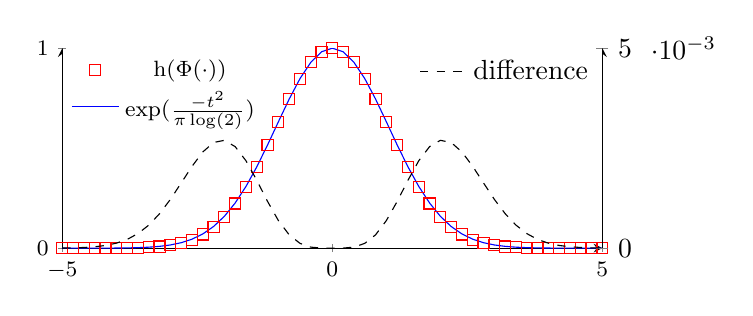
\begin{tikzpicture}

\begin{axis}[%
footnotesize,
scale only axis,
width=2.7in,
height=1.0in,
xmin=-5, xmax=5,
ymin=0, ymax=1,
xtick={-5,0,5},
ytick = {0,1},
axis y line = left,
axis x line = bottom,
legend style={ at={(0,1)}, anchor=north west, draw = none}]
]

\addplot [
color=red,
only marks,
mark=square,
mark options={solid}
]
coordinates{ (-5,6.64369e-06) (-4.8,1.72218e-05) (-4.6,4.2873e-05) (-4.4,0.000102503) (-4.2,0.000235365) (-4,0.000519064) (-3.8,0.0010995) (-3.6,0.00223711) (-3.4,0.00437257) (-3.2,0.00821083) (-3,0.0148147) (-2.8,0.0256873) (-2.6,0.0428103) (-2.4,0.0685917) (-2.2,0.105681) (-2,0.156615) (-1.8,0.223311) (-1.6,0.306444) (-1.4,0.40484) (-1.2,0.515021) (-1,0.631083) (-0.8,0.745014) (-0.6,0.847502) (-0.4,0.929133) (-0.2,0.981797) (0,1) (0.2,0.981797) (0.4,0.929133) (0.6,0.847502) (0.8,0.745014) (1,0.631083) (1.2,0.515021) (1.4,0.40484) (1.6,0.306444) (1.8,0.223311) (2,0.156615) (2.2,0.105681) (2.4,0.0685917) (2.6,0.0428103) (2.8,0.0256873) (3,0.0148147) (3.2,0.00821083) (3.4,0.00437257) (3.6,0.00223711) (3.8,0.0010995) (4,0.000519064) (4.2,0.000235365) (4.4,0.000102503) (4.6,4.2873e-05) (4.8,1.72218e-05) (5,6.64369e-06)
};
%\label{plots:approx_true}
\addlegendentry{$\mathrm{h}(\Phi(\cdot))$}

\addplot [
color=blue,
solid
]
coordinates{ (-5,1.03285e-05) (-4.8,2.54061e-05) (-4.6,6.02395e-05) (-4.4,0.00013768) (-4.2,0.000303323) (-4,0.000644146) (-3.8,0.00131859) (-3.6,0.00260182) (-3.4,0.0049487) (-3.2,0.00907298) (-3,0.0160344) (-2.8,0.0273151) (-2.6,0.0448534) (-2.4,0.0709961) (-2.2,0.108322) (-2,0.159311) (-1.8,0.22585) (-1.6,0.30863) (-1.4,0.406537) (-1.2,0.516189) (-1,0.631774) (-0.8,0.745348) (-0.6,0.847622) (-0.4,0.929159) (-0.2,0.981799) (0,1) (0.2,0.981799) (0.4,0.929159) (0.6,0.847622) (0.8,0.745348) (1,0.631774) (1.2,0.516189) (1.4,0.406537) (1.6,0.30863) (1.8,0.22585) (2,0.159311) (2.2,0.108322) (2.4,0.0709961) (2.6,0.0448534) (2.8,0.0273151) (3,0.0160344) (3.2,0.00907298) (3.4,0.0049487) (3.6,0.00260182) (3.8,0.00131859) (4,0.000644146) (4.2,0.000303323) (4.4,0.00013768) (4.6,6.02395e-05) (4.8,2.54061e-05) (5,1.03285e-05)
};
%\label{plots:approx_approx}
\addlegendentry{$\exp(\frac{-t^2}{\pi\log(2)})$}

\end{axis}

\begin{axis}[%
scale only axis,
width=2.7in,
height=1.0in,
xmin=-5, xmax=5,
ymin=0, ymax=0.005,
xtick={-5,0,5},
ytick = {0,0.005},
axis y line = right,
axis x line = none,
legend style={ at={(1,1)}, anchor=north east, draw = none}]
]

\addplot [
color=black,
dashed
]
coordinates{ (-5,3.68482e-06) (-4.8,8.18427e-06) (-4.6,1.73665e-05) (-4.4,3.51775e-05) (-4.2,6.79579e-05) (-4,0.000125081) (-3.8,0.000219088) (-3.6,0.000364708) (-3.4,0.000576126) (-3.2,0.000862153) (-3,0.00121977) (-2.8,0.00162773) (-2.6,0.00204316) (-2.4,0.00240434) (-2.2,0.0026417) (-2,0.00269602) (-1.8,0.00253851) (-1.6,0.00218519) (-1.4,0.00169772) (-1.2,0.00116807) (-1,0.000690885) (-0.8,0.000334143) (-0.6,0.000120243) (-0.4,2.60299e-05) (-0.2,1.71855e-06) (0,-0) (0.2,1.71855e-06) (0.4,2.60299e-05) (0.6,0.000120243) (0.8,0.000334143) (1,0.000690885) (1.2,0.00116807) (1.4,0.00169772) (1.6,0.00218519) (1.8,0.00253851) (2,0.00269602) (2.2,0.0026417) (2.4,0.00240434) (2.6,0.00204316) (2.8,0.00162773) (3,0.00121977) (3.2,0.000862153) (3.4,0.000576126) (3.6,0.000364708) (3.8,0.000219088) (4,0.000125081) (4.2,6.79579e-05) (4.4,3.51775e-05) (4.6,1.73665e-05) (4.8,8.18427e-06) (5,3.68482e-06)
};
%\label{plots:approx_error}
\addlegendentry{difference}

\end{axis}
\end{tikzpicture}
}
\caption{Analytic approximation to the binary entropy of the error function (\ref{plots:approx_true}) by a squared exponential (\ref{plots:approx_approx}). The absolute error (\ref{plots:approx_error}) remains under $3\cdot 10^{-3}$.}\label{fig:trick}
\end{figure}

where $C=\sqrt{\frac{\pi\ln2}{2}}$. Here, the first approximation, $\stackrel{1}{\approx}$, again reflects the Gaussian approximation to the posterior. The integral in the left hand side of Eqn.\ \eqref{eqn:mean_entropy} is hard to compute; $h(\Phi(t))$ must be integrated against a Gaussian distribution. However, inspection of the function $\mathrm{h}(\Phi(t))$ in Figure \ref{fig:trick} reveals that it is strikingly similar to a Gaussian shape $\exp(-t^2/\pi\ln2)$, the integration of which against a Gaussian is trivial. Indeed, the best fitting parameters can be validated by second order Taylor expansion of the logarithm of the function, also known as Laplace approximation. Thus, to approximate the mean entropy we replace $\mathrm{h}(\Phi(t))$ by $\exp(-t^2/\pi\log(2))$ and use the standard convolution formula for Gaussians to finally get Eqn.\ \eqref{eqn:mean_entropy}. We will refer to this approximation as $\stackrel{2}{\approx}$.

To summarise, the Bayesian Active Learning by Disagreement algorithm for Gaussian process classification consists of two steps. First it applies an approximate inference algorithm to obtain the posterior predictive mean $\mu_{\x,\data}$ and $\sigma_{\x,\data}$ for each point of interest $\x$. Then, it selects a query $\x$ that maximises the following objective function:

\begin{equation}
	\mathrm{h} \left( \Phi\left( \frac{\mu_{\x,\data}}{\sqrt{\sigma^2_{\x,\data} + 1}} \right)\right) - \frac{C \exp\left(-\frac{\mu_{\x,\data}^2}{2\left(\sigma_{\x,\data}^2 + C^2\right)}\right)}{\sqrt{\sigma_{\x,\data}^2 + C^2}} \tag{BALD-GPC}\label{eqn:BALD_GPC}
\end{equation}

The objective \eqref{eqn:BALD_GPC} is a smooth, differentiable function of $\x$, so gradient-based methods can be used to find the maximally informative query.

\section{Experiments}

This section shows our results on simulations that demonstrate the performance of BALD in Gaussian process classification. Although BALD can handle unconstrained search for informative queries in a continuous input space, we focus on pool-based active learning, whereby queries are restricted to a pre-defined pool $\mathcal{P}\in\mathcal{X}$ of unlabelled examples. We compare our algorithm to random sampling, maximum entropy sampling, query by committee using the deterministic vote criterion, and SVM active learning. In our experiments we also evaluated the informative vector machine (IVM) \cite{Lawrence04}, which is not an active learning algorithm in a strict sense. It is allowed to look at the label before selecting a query. The IVM has been introduced as a clever forward-selection algorithm for building sparse approximations to the posterior in GPC. We note that in fact, BALD could also be used in this context.

\begin{table}
\resizebox{3.25in}{!}{
\begin{tabular}{|c|c|c|c|}
\hline
&MCMC&EP ($\stackrel{1}{\approx}$)&Laplace ($\stackrel{1}{\approx}$)\\\hline
\hline
MC & 0 & $7.51\pm2.51$ & $41.57\pm4.02$ \\
approx ($\stackrel{2}{\approx}$)  & $0.16\pm0.05$ & $7.43\pm2.40$ & $40.45\pm3.67$ \\\hline
\end{tabular}
}
\label{tableinfoloss}
\caption{Percentage approximation error ($\pm$1 s.d.) \emph{Rows:} methods of approximate inference. \emph{Columns:} approximation methods for evaluating Eqn.\ \ref{eqn:mean_entropy}. The results indicate that $\stackrel{2}{\approx}$ is a very accurate approximation (Figure \ref{fig:trick}). EP causes some loss and Laplace significantly more, which is not surprising in the light of the results presented in \cite{Kuss05}.}
\end{table}

\subsection{Artificial Datasets}

\begin{figure*}[t]
\begin{center}
\begin{tabular}{rrr}
% This file was created by matlab2tikz v0.0.7.
% Copyright (c) 2008--2010, Nico Schlömer <nico.schloemer@gmail.com>
% All rights reserved.
% 
% The latest updates can be retrieved from
%   http://www.mathworks.com/matlabcentral/fileexchange/22022-matlab2tikz
% where you can also make suggestions and rate matlab2tikz.
% 
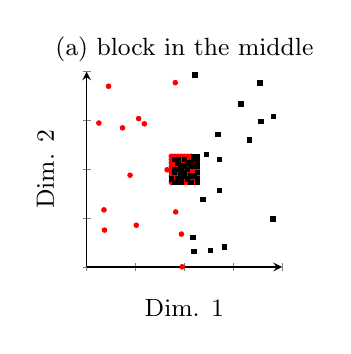
\begin{tikzpicture}

\begin{axis}[
footnotesize,
width= 1.6in,
height= 1.6in,
xmin=0, xmax=30,
ymin=0, ymax=30,
title={(a) block in the middle},
ytick={0,7.5,15,22.5,30},
xtick = {0,7.5,15,22.5,30},
xlabel = {Dim. 1},
ylabel = {Dim. 2},
xticklabels={,,,,},
yticklabels={,,,,},
axis on top,
axis y line = left,
axis x line = bottom
%legend entries={$optimal$,$rand$,$IVM$,$maxent$,$QBC2$,$QBC100$,$SVM$},
 %egend style={nodes=right}
]
\addplot [
color=red,
only marks,
mark=*,
mark options={scale = 0.4}
]
coordinates{ (13,13) (15,13) (15.5,13) (16.5,13) (13.5,13.5) (15,13.5) (16,13.5) (16.5,13.5) (13,14) (13.5,14) (14,14) (15.5,14) (17,14) (13,14.5) (14,14.5) (15.5,14.5) (16,14.5) (16.5,14.5) (13,15) (15,15) (16,15) (16.5,15) (17,15) (13,15.5) (13.5,15.5) (14,15.5) (15.5,15.5) (13,16) (13.5,16) (14.5,16) (15,16) (16.5,16) (13,16.5) (14.5,16.5) (15.5,16.5) (16,16.5) (13,17) (13.5,17) (14,17) (14.5,17) (15,17) (15.5,17) (16,17) (8.86203,21.9844) (1.87844,22.0987) (7.62888,6.41534) (5.50559,21.3585) (7.97933,22.783) (6.66413,14.0934) (2.66314,8.77752) (14.6582,0.0330902) (13.6696,8.46285) (2.74037,5.67331) (13.6087,28.3003) (12.3521,14.9273) (3.36577,27.7504) (14.5511,5.06006)
};
\label{plots:negatives}

\addplot [
color=black,
only marks,
mark=square*,
mark options={scale = 0.4}
]
coordinates{ (13.5,13) (14,13) (14.5,13) (16,13) (17,13) (13,13.5) (14,13.5) (14.5,13.5) (15.5,13.5) (17,13.5) (14.5,14) (15,14) (16,14) (16.5,14) (13.5,14.5) (14.5,14.5) (15,14.5) (17,14.5) (13.5,15) (14,15) (14.5,15) (15.5,15) (14.5,15.5) (15,15.5) (16,15.5) (16.5,15.5) (17,15.5) (14,16) (15.5,16) (16,16) (17,16) (13.5,16.5) (14,16.5) (15,16.5) (16.5,16.5) (17,16.5) (16.5,17) (17,17) (18.3773,17.3043) (24.9794,19.4896) (26.7589,22.3496) (17.8888,10.3495) (16.4577,2.38458) (20.4057,11.7607) (19.0268,2.51172) (20.4262,16.5161) (28.71,23.0737) (21.1403,3.08034) (16.3379,4.55224) (20.1516,20.3166) (23.7032,25.0623) (26.6266,28.273) (16.6152,29.476) (28.6434,7.37318)
};
\label{plots:positives}

\end{axis}
\end{tikzpicture}
&
% This file was created by matlab2tikz v0.0.7.
% Copyright (c) 2008--2010, Nico Schlömer <nico.schloemer@gmail.com>
% All rights reserved.
% 
% The latest updates can be retrieved from
%   http://www.mathworks.com/matlabcentral/fileexchange/22022-matlab2tikz
% where you can also make suggestions and rate matlab2tikz.
% 
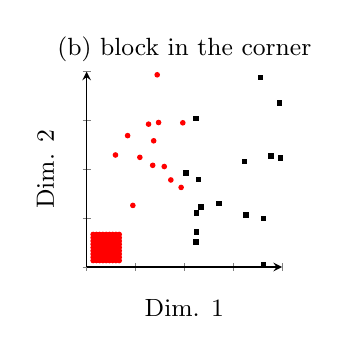
\begin{tikzpicture}

\begin{axis}[
footnotesize,
width= 1.6in,
height= 1.6in,
xmin=0, xmax=30,
ymin=0, ymax=30,
title={(b) block in the corner},
xlabel = {Dim. 1},
ylabel = {Dim. 2},
ytick={0,7.5,15,22.5,30},
xtick = {0,7.5,15,22.5,30},
xticklabels={,,,,},
yticklabels={,,,,},
axis on top,
axis y line = left,
axis x line = bottom
%legend entries={$optimal$,$rand$,$IVM$,$maxent$,$QBC2$,$QBC100$,$SVM$},
 %egend style={nodes=right}
]

\addplot [
color=red,
only marks,
mark=*,
mark options={scale=0.4}
]
coordinates{ (1,1) (1.5,1) (2,1) (2.5,1) (3,1) (3.5,1) (4,1) (4.5,1) (5,1) (1,1.5) (1.5,1.5) (2,1.5) (2.5,1.5) (3,1.5) (3.5,1.5) (4,1.5) (4.5,1.5) (5,1.5) (1,2) (1.5,2) (2,2) (2.5,2) (3,2) (3.5,2) (4,2) (4.5,2) (5,2) (1,2.5) (1.5,2.5) (2,2.5) (2.5,2.5) (3,2.5) (3.5,2.5) (4,2.5) (4.5,2.5) (5,2.5) (1,3) (1.5,3) (2,3) (2.5,3) (3,3) (3.5,3) (4,3) (4.5,3) (5,3) (1,3.5) (1.5,3.5) (2,3.5) (2.5,3.5) (3,3.5) (3.5,3.5) (4,3.5) (4.5,3.5) (5,3.5) (1,4) (1.5,4) (2,4) (2.5,4) (3,4) (3.5,4) (4,4) (4.5,4) (5,4) (1,4.5) (1.5,4.5) (2,4.5) (2.5,4.5) (3,4.5) (3.5,4.5) (4,4.5) (4.5,4.5) (5,4.5) (1,5) (1.5,5) (2,5) (2.5,5) (3,5) (3.5,5) (4,5) (4.5,5) (5,5) (14.7594,22.137) (9.50211,21.9321) (11.9146,15.4247) (4.42475,17.1991) (7.09258,9.45929) (11.0419,22.1845) (14.5021,12.2209) (12.9235,13.3655) (10.8308,29.5065) (10.2906,19.3776) (4.33421,3.57372) (10.1417,15.6132) (6.28981,20.1691) (8.16591,16.8388)
};

\addplot [
color=black,
only marks,
mark=square*,
mark options={scale=0.4}
]
coordinates{ (17.1549,13.4394) (29.7725,16.7571) (16.7772,22.7654) (28.2901,17.0776) (16.8774,8.28907) (17.5203,9.19147) (27.1422,7.43214) (16.8312,5.41786) (20.3286,9.78169) (24.4829,8.00663) (27.1345,0.366002) (29.6109,25.1893) (24.263,16.1932) (15.2474,14.4045) (26.6495,29.111) (16.7822,3.87225)
};

\end{axis}
\end{tikzpicture}
&
% This file was created by matlab2tikz v0.0.7.
% Copyright (c) 2008--2010, Nico Schlömer <nico.schloemer@gmail.com>
% All rights reserved.
% 
% The latest updates can be retrieved from
%   http://www.mathworks.com/matlabcentral/fileexchange/22022-matlab2tikz
% where you can also make suggestions and rate matlab2tikz.
% 
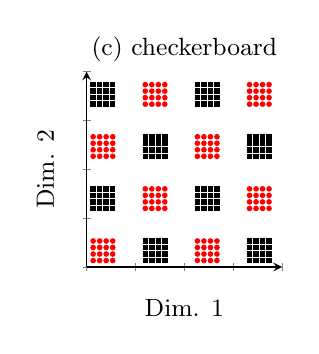
\begin{tikzpicture}

\begin{axis}[
footnotesize,
width= 1.6in,
height= 1.6in,
xmin=0, xmax=30,
ymin=0, ymax=30,
title={(c) checkerboard},
xlabel = {Dim. 1},
ylabel = {Dim. 2},
ytick={0,7.5,15,22.5,30},
xtick = {0,7.5,15,22.5,30},
xticklabels={,,,,},
yticklabels={,,,,},
axis on top,
axis y line = left,
axis x line = bottom
%legend entries={$optimal$,$rand$,$IVM$,$maxent$,$QBC2$,$QBC100$,$SVM$},
 %egend style={nodes=right}
]

\addplot [
color=red,
only marks,
mark=*,
mark options={scale=0.4}
]
coordinates{ (1,1) (2,1) (3,1) (4,1) (17,1) (18,1) (19,1) (20,1) (1,2) (2,2) (3,2) (4,2) (17,2) (18,2) (19,2) (20,2) (1,3) (2,3) (3,3) (4,3) (17,3) (18,3) (19,3) (20,3) (1,4) (2,4) (3,4) (4,4) (17,4) (18,4) (19,4) (20,4) (9,9) (10,9) (11,9) (12,9) (25,9) (26,9) (27,9) (28,9) (9,10) (10,10) (11,10) (12,10) (25,10) (26,10) (27,10) (28,10) (9,11) (10,11) (11,11) (12,11) (25,11) (26,11) (27,11) (28,11) (9,12) (10,12) (11,12) (12,12) (25,12) (26,12) (27,12) (28,12) (1,17) (2,17) (3,17) (4,17) (17,17) (18,17) (19,17) (20,17) (1,18) (2,18) (3,18) (4,18) (17,18) (18,18) (19,18) (20,18) (1,19) (2,19) (3,19) (4,19) (17,19) (18,19) (19,19) (20,19) (1,20) (2,20) (3,20) (4,20) (17,20) (18,20) (19,20) (20,20) (9,25) (10,25) (11,25) (12,25) (25,25) (26,25) (27,25) (28,25) (9,26) (10,26) (11,26) (12,26) (25,26) (26,26) (27,26) (28,26) (9,27) (10,27) (11,27) (12,27) (25,27) (26,27) (27,27) (28,27) (9,28) (10,28) (11,28) (12,28) (25,28) (26,28) (27,28) (28,28)
};

\addplot [
color=black,
only marks,
mark=square*,
mark options={scale=0.4}
]
coordinates{ (9,1) (10,1) (11,1) (12,1) (25,1) (26,1) (27,1) (28,1) (9,2) (10,2) (11,2) (12,2) (25,2) (26,2) (27,2) (28,2) (9,3) (10,3) (11,3) (12,3) (25,3) (26,3) (27,3) (28,3) (9,4) (10,4) (11,4) (12,4) (25,4) (26,4) (27,4) (28,4) (1,9) (2,9) (3,9) (4,9) (17,9) (18,9) (19,9) (20,9) (1,10) (2,10) (3,10) (4,10) (17,10) (18,10) (19,10) (20,10) (1,11) (2,11) (3,11) (4,11) (17,11) (18,11) (19,11) (20,11) (1,12) (2,12) (3,12) (4,12) (17,12) (18,12) (19,12) (20,12) (9,17) (10,17) (11,17) (12,17) (25,17) (26,17) (27,17) (28,17) (9,18) (10,18) (11,18) (12,18) (25,18) (26,18) (27,18) (28,18) (9,19) (10,19) (11,19) (12,19) (25,19) (26,19) (27,19) (28,19) (9,20) (10,20) (11,20) (12,20) (25,20) (26,20) (27,20) (28,20) (1,25) (2,25) (3,25) (4,25) (17,25) (18,25) (19,25) (20,25) (1,26) (2,26) (3,26) (4,26) (17,26) (18,26) (19,26) (20,26) (1,27) (2,27) (3,27) (4,27) (17,27) (18,27) (19,27) (20,27) (1,28) (2,28) (3,28) (4,28) (17,28) (18,28) (19,28) (20,28)
};

\end{axis}
\end{tikzpicture}
\\
\input{figures/blockinthemiddle.tikz}&
\input{figures/corner.tikz}&
% This file was created by matlab2tikz v0.0.7.
% Copyright (c) 2008--2010, Nico Schlömer <nico.schloemer@gmail.com>
% All rights reserved.
% 
% The latest updates can be retrieved from
%   http://www.mathworks.com/matlabcentral/fileexchange/22022-matlab2tikz
% where you can also make suggestions and rate matlab2tikz.
% 
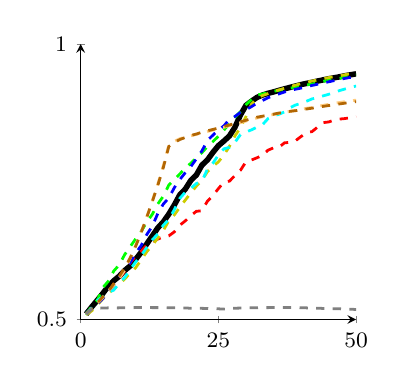
\begin{tikzpicture}

% defining custom colors
\definecolor{mycolor1}{rgb}{0.8,0.8,0}
\definecolor{mycolor2}{rgb}{0,1,1}
\definecolor{mycolor3}{rgb}{1,0.8,0.5}
\definecolor{mycolor4}{rgb}{0.7,0.4,0.01}


\begin{axis}[
footnotesize,
width= 2in,
height= 2in,
xmin=0, xmax=50,
ymin=0.5, ymax=1,
ytick={0.5,1},
xtick = {0,25,50},
axis on top,
axis y line = left,
axis x line = bottom
%legend entries={$optimal$,$rand$,$IVM$,$maxent$,$QBC2$,$QBC100$,$SVM$},
 %egend style={nodes=right}
]

\addplot [
color=black,
solid,
line width=2.0pt
]
coordinates{ (1,0.509885) (2,0.522693) (3,0.53474) (4,0.547013) (5,0.560323) (6,0.57036) (7,0.57857) (8,0.589043) (9,0.597232) (10,0.609322) (11,0.622262) (12,0.637122) (13,0.651602) (14,0.66623) (15,0.677149) (16,0.691247) (17,0.707813) (18,0.726329) (19,0.736819) (20,0.752558) (21,0.762286) (22,0.780063) (23,0.789513) (24,0.803286) (25,0.815501) (26,0.823959) (27,0.833154) (28,0.848929) (29,0.87118) (30,0.888573) (31,0.896232) (32,0.903101) (33,0.907358) (34,0.910533) (35,0.913087) (36,0.915929) (37,0.918698) (38,0.921288) (39,0.923818) (40,0.926381) (41,0.928526) (42,0.930591) (43,0.932818) (44,0.9349) (45,0.936965) (46,0.938718) (47,0.94052) (48,0.942503) (49,0.944208) (50,0.945905)
};

\addplot [
color=red,
dashed,
line width=1.0pt
]
coordinates{ (1,0.509773) (2,0.519229) (3,0.528577) (4,0.538652) (5,0.548848) (6,0.56459) (7,0.573944) (8,0.588079) (9,0.603113) (10,0.615583) (11,0.624322) (12,0.635052) (13,0.640151) (14,0.646008) (15,0.649586) (16,0.651762) (17,0.659059) (18,0.671112) (19,0.679088) (20,0.688642) (21,0.696339) (22,0.697418) (23,0.714628) (24,0.724863) (25,0.737618) (26,0.749363) (27,0.751161) (28,0.761194) (29,0.770765) (30,0.786319) (31,0.789465) (32,0.793527) (33,0.798071) (34,0.807288) (35,0.81155) (36,0.812729) (37,0.820657) (38,0.821573) (39,0.824516) (40,0.83211) (41,0.839197) (42,0.84107) (43,0.849292) (44,0.857284) (45,0.858584) (46,0.861788) (47,0.863781) (48,0.864775) (49,0.86646) (50,0.867783)
};

\addplot [
color=green,
dashed,
line width=1.0pt
]
coordinates{ (1,0.508449) (2,0.52448) (3,0.534489) (4,0.557607) (5,0.569195) (6,0.587917) (7,0.599197) (8,0.617996) (9,0.632287) (10,0.646611) (11,0.660148) (12,0.676873) (13,0.69087) (14,0.709665) (15,0.723865) (16,0.744137) (17,0.75402) (18,0.764207) (19,0.774987) (20,0.783602) (21,0.7938) (22,0.802727) (23,0.813786) (24,0.822881) (25,0.832758) (26,0.843949) (27,0.855273) (28,0.867317) (29,0.877196) (30,0.889835) (31,0.899085) (32,0.907538) (33,0.909411) (34,0.911749) (35,0.91423) (36,0.916021) (37,0.917998) (38,0.919709) (39,0.922173) (40,0.924) (41,0.925656) (42,0.927179) (43,0.930009) (44,0.93237) (45,0.933966) (46,0.935606) (47,0.937825) (48,0.940095) (49,0.941935) (50,0.943745)
};

\addplot [
color=mycolor1,
dashed,
line width=1.0pt
]
coordinates{ (1,0.508616) (2,0.515568) (3,0.525883) (4,0.537191) (5,0.547513) (6,0.554742) (7,0.564037) (8,0.573611) (9,0.584294) (10,0.594309) (11,0.60828) (12,0.622964) (13,0.634804) (14,0.647751) (15,0.661483) (16,0.67922) (17,0.689835) (18,0.703799) (19,0.716897) (20,0.729839) (21,0.74205) (22,0.752144) (23,0.768311) (24,0.778327) (25,0.786078) (26,0.798597) (27,0.814074) (28,0.833299) (29,0.848099) (30,0.868333) (31,0.89076) (32,0.901281) (33,0.906562) (34,0.90999) (35,0.913697) (36,0.916841) (37,0.919672) (38,0.922692) (39,0.925409) (40,0.928351) (41,0.930613) (42,0.9328) (43,0.934905) (44,0.937044) (45,0.939053) (46,0.940839) (47,0.942414) (48,0.944379) (49,0.94623) (50,0.947845)
};

\addplot [
color=mycolor2,
dashed,
line width=1.0pt
]
coordinates{ (1,0.511368) (2,0.521234) (3,0.534471) (4,0.541192) (5,0.549296) (6,0.55336) (7,0.566196) (8,0.576368) (9,0.590969) (10,0.604769) (11,0.616152) (12,0.631036) (13,0.644519) (14,0.655425) (15,0.671102) (16,0.681668) (17,0.699288) (18,0.719853) (19,0.731265) (20,0.738205) (21,0.746837) (22,0.750747) (23,0.772712) (24,0.783562) (25,0.798642) (26,0.80975) (27,0.812511) (28,0.821576) (29,0.835568) (30,0.840282) (31,0.8442) (32,0.849221) (33,0.853489) (34,0.86456) (35,0.869843) (36,0.872548) (37,0.87679) (38,0.88439) (39,0.889286) (40,0.892362) (41,0.896182) (42,0.900409) (43,0.902785) (44,0.905872) (45,0.908694) (46,0.911805) (47,0.915563) (48,0.918425) (49,0.921418) (50,0.923699)
};

\addplot [
color=blue,
dashed,
line width=1.0pt
]
coordinates{ (1,0.509498) (2,0.519054) (3,0.527929) (4,0.537568) (5,0.551151) (6,0.56285) (7,0.576111) (8,0.592502) (9,0.603575) (10,0.62071) (11,0.634414) (12,0.654218) (13,0.669335) (14,0.692337) (15,0.70947) (16,0.720645) (17,0.739182) (18,0.754014) (19,0.766625) (20,0.777609) (21,0.791608) (22,0.805876) (23,0.825049) (24,0.834503) (25,0.844029) (26,0.851438) (27,0.863511) (28,0.868529) (29,0.875978) (30,0.881048) (31,0.886339) (32,0.892711) (33,0.897363) (34,0.902574) (35,0.90609) (36,0.909593) (37,0.91294) (38,0.916156) (39,0.917961) (40,0.920041) (41,0.922319) (42,0.924864) (43,0.927053) (44,0.929225) (45,0.931453) (46,0.933538) (47,0.935713) (48,0.93771) (49,0.939482) (50,0.941397)
};

\addplot [
color=mycolor3,
dashed,
line width=1.0pt
]
coordinates{ (1,0.509503) (2,0.519416) (3,0.529021) (4,0.539572) (5,0.550976) (6,0.562576) (7,0.575101) (8,0.589434) (9,0.611601) (10,0.634933) (11,0.659819) (12,0.686802) (13,0.715388) (14,0.745879) (15,0.779305) (16,0.81661) (17,0.823452) (18,0.828173) (19,0.830868) (20,0.83343) (21,0.836034) (22,0.838609) (23,0.8412) (24,0.843833) (25,0.846406) (26,0.848906) (27,0.851831) (28,0.854557) (29,0.857288) (30,0.860204) (31,0.863002) (32,0.8658) (33,0.867865) (34,0.87011) (35,0.872043) (36,0.874039) (37,0.875788) (38,0.877721) (39,0.879712) (40,0.881449) (41,0.883304) (42,0.884793) (43,0.88689) (44,0.888692) (45,0.890531) (46,0.89233) (47,0.893886) (48,0.895479) (49,0.896751) (50,0.89818)
};

\addplot [
color=mycolor4,
dashed,
line width=1.0pt
]
coordinates{ (1,0.5108) (2,0.519728) (3,0.529965) (4,0.540986) (5,0.551291) (6,0.564799) (7,0.577927) (8,0.594231) (9,0.611973) (10,0.633352) (11,0.658299) (12,0.685346) (13,0.714151) (14,0.743465) (15,0.775744) (16,0.814025) (17,0.821312) (18,0.826681) (19,0.830442) (20,0.833942) (21,0.836694) (22,0.839855) (23,0.842425) (24,0.845011) (25,0.847563) (26,0.850202) (27,0.853042) (28,0.855901) (29,0.858893) (30,0.861653) (31,0.864464) (32,0.867183) (33,0.869036) (34,0.870872) (35,0.872713) (36,0.874727) (37,0.876214) (38,0.877867) (39,0.878996) (40,0.880543) (41,0.882084) (42,0.883558) (43,0.885244) (44,0.886777) (45,0.888309) (46,0.889937) (47,0.891268) (48,0.892703) (49,0.894114) (50,0.895325)
};

\addplot [
color=gray,
dashed,
line width=1.0pt
]
coordinates{ (1,0.509276) (2,0.519678) (3,0.520474) (4,0.520784) (5,0.521128) (6,0.520995) (7,0.521126) (8,0.521426) (9,0.521438) (10,0.521617) (11,0.521681) (12,0.521675) (13,0.521558) (14,0.521564) (15,0.521527) (16,0.521368) (17,0.521186) (18,0.520923) (19,0.520794) (20,0.520524) (21,0.520356) (22,0.520213) (23,0.520105) (24,0.519821) (25,0.519346) (26,0.519055) (27,0.520018) (28,0.520581) (29,0.520693) (30,0.521041) (31,0.521272) (32,0.521516) (33,0.521537) (34,0.521562) (35,0.521635) (36,0.521661) (37,0.521637) (38,0.521593) (39,0.521533) (40,0.521368) (41,0.521099) (42,0.52069) (43,0.520444) (44,0.520095) (45,0.519873) (46,0.519582) (47,0.519396) (48,0.518945) (49,0.518611) (50,0.518228)
};

\end{axis}
\end{tikzpicture}
\\
\end{tabular}
\end{center}
\caption{\emph{Top:} Artificial datasets used in our evaluation of active learning methods. Exemplars of the two classes are shown with black squares (\ref{plots:positives}) and red circles(\ref{plots:negatives}). \emph{Bottom:} Results of active learning with seven methods: random query (\ref{plots:rand}), BALD (\ref{plots:BALD}),  maximum entropy sampling (\ref{plots:maxent}), query by committee with the vote criterion with 2 ($\mbox{QBC}_2$, \ref{plots:QBC2}) and 100 ($\mbox{QBC}_{100}$, \ref{plots:QBC100}) committee members, active SVM (\ref{plots:SVM}) and IVM (\ref{plots:IVM}).}
\label{fig:artificial}
\end{figure*}

The algorithms were tested on three highly artificial, but challenging, datasets. The first of which is similar to the \texttt{checkerboard} dataset used in \cite{chu2005preference}, and is designed to test the algorithm's capabilities to find multiple disjoint islands of points from one class. The second, \texttt{block in the corner}, has a block of uninformative points far from the decision boundary, and the third, \texttt{block in the middle}, has a block of noisy points on the decision boundary: a strong active learning algorithm should avoid these uninformative regions. The three datasets are depicted in Figure\ref{fig:artificial}.

\subsection{Real Datasets}

We present results on three real world datasets also, one of which is a preference learning. The two classification datasets are: determining the gender of Leptograspus crabs (\texttt{crabs})\footnote{Data set at http://archive.ics.uci.edu/ml/datasets/} and diagnosis of malignant Breast Cancer cells (\texttt{cancer})\footnote{Data set at http://www.stats.ox.ac.uk/pub/PRNN/}. For preference elicitation we use BALD in the GP-based model proposed by \cite{chu2005preference} which is formally equivalent to GPC with an appropriately chosen covariance function (see supplementary for details). We evaluate this method on the \texttt{cpu preference} dataset introduced in \cite{chu2005preference}.

We also investigate the detriment in performance when datasets are corrupted or made more difficult. We present two scenarios, both using the \texttt{cancer} dataset. In the first pool, points are mislabelled with probability 0.1; in the second, training data is removed from one class, so that the pool has a 4:1 class inbalance.

\subsection{Results}

\paragraph{Quantifying Approximation Losses:} To obtain \eqref{eqn:BALD_GPC} we made two approximations: we perform approximate inference ($\stackrel{1}{\approx}$), and we approximated the binary entropy of the Gaussian CDF by a squared exponential ($\stackrel{2}{\approx}$). Both of these can be substituted with Monte Carlo approximation, enabling us to compute an asymptotically unbiased estimate of the expected information gain. Using extensive Monte Carlo as the `gold standard', we can evaluate how much we loose by applying these approximations. We use the following measure to quantify the approximation error:
\begin{equation}
	\frac{\max_{\x\in\mathcal{P}}I(\x) - I(\argmax_{\x\in\mathcal{P}}\hat{I}(x))}{\max_{\x\in\mathcal{P}}I(\x) }\cdot 100\%
\end{equation}
where $I$ is the objective computed using Monte Carlo, $\hat{I}$ is the approximate objective. These experiments were run on the \texttt{cancer} dataset, results are shown and discussed in Table \ref{tableinfoloss}.

\paragraph{Pool-based active learning:} In most scenarios, BALD is amongst the best performing methods and is often the best. It successfully finds the disjoint regions in the \texttt{checkerboard} quickly and avoids the uninformative `blocks' in the other artificial datasets. The IVM, as expected, is unable to cope with noisy datasets because, using lookahead, it targets the `interesting' mislabelled points, yielding a highly biased training set. The SVM also targets pathological points in the noisy dataset and surprisingly performs very poorly with the crabs dataset. Maximum entropy sampling sometimes performs as well as an approximation to BALD; however, in other situations its performance tails off as it starts repeatedly querying points where the output is inherently uncertain (see Section 3.2). This is particularly noticeable in the \texttt{block in the middle} dataset (as expected) and the \texttt{crabs} dataset. It must be noted that maximum entropy sampling benefits greatly from the pool-based scenario. As each point in a pool can be queried only once, the algorithm is forced to explore the space better. Maximum entropy sampling would perform much worse, if query points could be selected without constraints. Query by committee performs reasonably well across datasets. Interestingly, having only 2 committee members often proved better, than having 100.

\begin{table*}
\begin{center}
\resizebox{6.75in}{!}{
\begin{tabular}{|l|ccccccc|}
\hline
Dataset&BALD \ref{plots:BALD}&random \ref{plots:rand}&max ent \ref{plots:maxent}&$\mbox{QBC}_{2}$ \ref{plots:QBC2}&$\mbox{QBC}_{100}$\ref{plots:QBC100}&IVM \ref{plots:IVM}&active SVM \ref{plots:SVM}\\\noalign{\hrule height 1.2pt}
\texttt{cancer}&$\bm{31.5\pm1.8^{\textcolor{red}{\star}}}$&$\bm{40.0\pm10.3}$&$47.3\pm3.1$&$\bm{36.4\pm10.3}$&$37.2\pm3.1$&N/A&$42.1\pm3.4$\\
\texttt{cancer}$_{noisy}$&$17.2\pm4.4$&$\bm{16.6\pm10.2}$&$24.9\pm8.5$&$\bm{12.2\pm2.9^{\textcolor{red}{\star}}}$&$20.6\pm2.6$&N/A&N/A\\
\texttt{cancer}$_{unbalanced}$&$\bm{ 8.5\pm5.0^{\textcolor{red}{\star}}}$&$30.6\pm13.5$&$\bm{11.2\pm7.5}$&$\bm{24.6\pm17.0}$&$14.8\pm1.8$&$35.8\pm5.9$&$41.4\pm0.5$\\
\texttt{crabs}&$\bm{20.9\pm4.5^{\textcolor{red}{\star}}}$&$29.1\pm5.4$&$34.7\pm9.2$&$28.6\pm4.0$&$\bm{22.4\pm4.3}$&$26.7\pm2.2$&$40.6\pm8.6$\\
\texttt{cpu-pref}&$\bm{68.9\pm24.6^{\textcolor{red}{\star}}}$&$192.9\pm34.8$&$181.3\pm8.1$&$211.0\pm69.3$&$286.0\pm12.1$&$159.3\pm1.2$&$184.7\pm2.3$\\
\texttt{block middle}&$\bm{20.7\pm6.3^{\textcolor{red}{\star}}}$&$43.7\pm2.2$&$\bm{32.8\pm14.8}$&$\bm{33.0\pm17.9}$&$40.0\pm7.4$&N/A&$\bm{27.9\pm9.2}$\\
\texttt{block corner}&$\bm{ 9.7\pm0.5^{\textcolor{red}{\star}}}$&$32.1\pm3.4$&$10.1\pm0.3$&$10.9\pm0.3$&$11.4\pm0.8$&$14.3\pm0.9$&$14.0\pm1.2$\\
\texttt{checkerboard}&$\bm{55.0\pm0.0^{\textcolor{red}{\star}}}$&$110.8\pm10.5$&$56.4\pm0.9$&$89.0\pm1.4$&$70.8\pm1.8$&$56.0\pm0.0$&$65.4\pm7.3$\\
\hline
\end{tabular}
}
\caption{Performance of active learning algorithms for GPC across several datasets. The nubmers shown are the average number of datapoints required to achieve $98\%$ of the accuracy achieved on the whole pool (lower is better). The best method for each dataset is denoted by $^{\textcolor{red}{\star}}$, those that come within one standard deviation to the best are highlighted in bold. `N/A' indicates if the method did not reach the $98\%$ performance level during our simulations. BALD outperforms other methods or is among the best in all datasets except for \texttt{cancer}$_{noisy}$, where extra label noise was added. The gain is particularly large in the case of the \texttt{cpu-pref} dataset.}
\label{bigtable}
\end{center}
\end{table*}

%\begin{table}
 %\pgfplotstabletypeset[outfile={data.out},every head row/.style={before row=\hline,after row=\hline\hline}, every last row/.style={after row=\hline}, every first column/.style={column type/.add={|}},every even row/.style={ before row={\rowcolor[gray]{0.9}}}]{data/results-real-errorbars.dat}
%\end{table}
\begin{figure*}
\begin{center}
\begin{tabular}{rrr}
\input{figures/cancer_normal.tikz}&
\input{figures/cancer_unbalanced.tikz}&
\input{figures/cancer_noise.tikz}\\
\input{figures/cancer_SVM.tikz}&
\input{figures/cancer_unbalanced_SVM.tikz}&
\input{figures/cancer_noise_SVM.tikz}\\
\end{tabular}
\end{center}
\caption{Classification accuracy in the \texttt{cancer} dataset shown for 7 active learning strategies:
random query (\ref{plots:rand}), BALD (\ref{plots:BALD}),  maximum entropy
sampling (\ref{plots:maxent}), query by committee with the vote criterion with
2 ($\mbox{QBC}_2$, \ref{plots:QBC2}) and 100 ($\mbox{QBC}_{100}$,
\ref{plots:QBC100}) committee members, active SVM (\ref{plots:SVM}) and IVM (\ref{plots:IVM}).
(a--c) show the probability of correct response in GPC, in (d--f) shows the percentage of correct predictions by an SVM.}
\label{fig:cancer}
\end{figure*}

\section{Discussion}

\paragraph{Summary} We motivated an information theoretic approach to active learning to yield a learner that is not tied to any domain or loss function. We further motivated Shannon's Entropy of the parameter posterior as a sensible measure of uncertainty.  We note that the reformulation in \eqref{eqn:info2} is critical in forming a tractable objective function and showed that the informativeness can be expressed in terms of a Bayesian principle of maximal disagreement, and proposed a framework that we call BALD.  We made theoretical connections between BALD and maximum entropy sampling, version space minimisation, query by committee and the Informative Vector Machine.  In the second part of the paper we focused on applying the general methodology in Gaussian Process classification and developed a novel and tractable objective function for active learning in GPC. For this, we suggested and analytic trick that yields a tractable approximation to the binary entropy of the Gaussian CDF. Our method can be used with a wide range of approximate inference methods; expectation propagation, combined with our analytic criterion \eqref{eqn:BALD_GPC} represents an sensible trade-off between accuracy and efficiency.

\paragraph{Further Investigation} We note from Table \ref{bigtable} that BALD significantly outperforms other methodologies in the preference learning domain; this motivates the application of BALD to harder preference learning problems, and domains with more complicated input or output structure. Other possible studies include BALD's application to unconstrained queries in a continuous space, where one must design an efficient optimisation algorithm to cope with an ever increasing number of local maxima. More generally, the development of tractable decision theoretic approaches to active learning is a new, and exciting, area of research. We plan to investigate how much of the BALD reformulation can be generalised to other loss functions.

{\small
\bibliographystyle{veryshort}
\bibliography{bib/bibliog}
}


\end{document}
